\documentclass[10pt]{article}
\usepackage[margin=0.72in]{geometry}
\usepackage{booktabs}
\usepackage{hyperref}
\usepackage{tikz}

\hypersetup{colorlinks=true, urlcolor=blue, linkcolor=black, citecolor=black}
\setlength{\parskip}{0.35em}
\setlength{\parindent}{0pt}

\title{\vspace{-1.2em}Training Through the Inferno: An Inspectable OSRS Boss-Fight Benchmark for RL\vspace{-0.4em}}
\author{Anonymous Authors}
\date{}

\begin{document}
\maketitle
\vspace{-1.8em}

\begin{abstract}
We argue that modern game RL benchmarks benefit from three properties: fast training, inspectable failures, and enough simulator fidelity that policy mistakes mean something. We present an Old School RuneScape Inferno benchmark built in PufferLib 4. The Inferno is a 69-wave solo boss encounter with prayer switching, line-of-sight positioning, supplies, target priority, and a moving-shield final phase. These mechanics create long episodes, partial observability, sparse success, and failure modes designed to be readable by skilled players.

The contribution is a benchmark design pattern: player-readable state, structured actions, strict masks, replayable failures, behavior-level logs, and high-throughput recurrent training. The environment exposes 744 symbolic observation features, 9 action heads, and 89 mask logits. We use PufferLib 4's native recurrent RL stack to make large-agent, long-episode iteration practical. A compact recurrent checkpoint trained for 171.7M environment steps reached 0.49 logged development win rate and 0.736 internal progress score in the stored run summary. The stored run summary shows that this benchmark version can train a policy with logged full clears while retaining late-fight diagnostic counters for healer progress, prayer correctness, and Zuk HP. It is not evidence of a solved benchmark.
\end{abstract}

\section{Introduction and Contribution}

The Old School RuneScape Inferno is a solo player-versus-monster challenge released in 2017. The player must survive 69 waves and defeat TzKal-Zuk to earn the infernal cape. The OSRS Wiki describes the activity as a no-restock encounter with three pillars that block projectiles during the waves and a mandatory shield mechanic in the final fight \cite{osrs-inferno}. This makes the Inferno useful for game RL because many failures are player-readable. If the agent dies to a Jal-Zek, it may have missed a magic prayer. If a pillar falls, it likely ignored nibblers. If Zuk shield health drops, it failed movement, target priority, or healer timing.

This paper is about benchmark construction. We do not wrap a game binary and report a leaderboard number. We build a simulator whose state, actions, masks, renderer, replay path, and logs form one contract. The same game facts used for training should be available when explaining watched behavior. If a policy looks wrong in replay, the logs and simulator should explain why.

The benchmark fits RLVG along three axes. First, it is a modern game-derived task with long-horizon resource management and timing. Second, it supports behavioral evaluation: the benchmark exposes whether policy behavior matches player-readable task structure when scalar reward rises. Third, it depends on systems work. The environment became useful only when it could train, render, and replay fast enough to make debugging empirical.

\section{Benchmark Surface}

The Inferno environment uses symbolic observations instead of pixels. The current surface has 744 observation features, 9 action heads, and 89 action mask logits. One environment step is one OSRS game tick, or 0.6 seconds. Episodes can run for thousands of ticks. The native environment writes fixed-size observations and masks into PufferLib rollout buffers for thousands of parallel agents.

The observation vector contains player health, prayer, supplies, wave phase, gear state, combat stats, target state, weapon range, NPC slots, pillar health, pending hits, pending Zuk healer area attacks, and short movement forecasts. Positions are normalized and mostly egocentric or arena-relative. Categories use one-hot structure or slot membership. The design rule is simple: expose player-relevant state, then log whether the policy acts on it.

The action space is a structured interface over OSRS intent: movement, overhead prayer, target selection, gear switching, food, potion, spell, special attack, and offensive prayer. The target head points into observation slots instead of raw entity ids. The mask writer validates every action head and records zero-valid-head failures. Invalid actions are interface noise. The model should decide whether to run west, pray magic, tag a healer, cast barrage, or drink a restore. It should spend capacity on game decisions, not on learning that an absent NPC cannot be attacked.

\begin{table}[t]
\centering
\small
\begin{tabular}{lll}
\toprule
Component & Design choice & Why it matters \\
\midrule
Observation & 744 symbolic features & Exposes player-relevant state \\
Action & 9 structured heads & Matches game intent \\
Masks & 89 strict mask logits & Removes invalid client actions \\
Debug & Renderer, replay, logs & Makes failures inspectable \\
Training & 4096 parallel agents & Keeps long episodes cheap \\
Evaluation & Normal-start summary & Separates full-run progress \\
\bottomrule
\end{tabular}
\caption{The benchmark surface is designed so training, replay, masks, and logs refer to the same game facts.}
\label{tab:surface}
\end{table}

Reward and score are separate. Reward can be shaped, swept, and replaced. Score is intended to survive those edits. In this environment, reward paid for credit assignment through damage, healer tags, shield preservation, late-wave pressure, and final-phase priorities. The reported score is an internal development progress metric: a win returns 2.0, while partial runs receive Zuk HP progress plus late-fight milestone bonuses.

\begin{figure}[t]
\centering
\resizebox{0.95\linewidth}{!}{
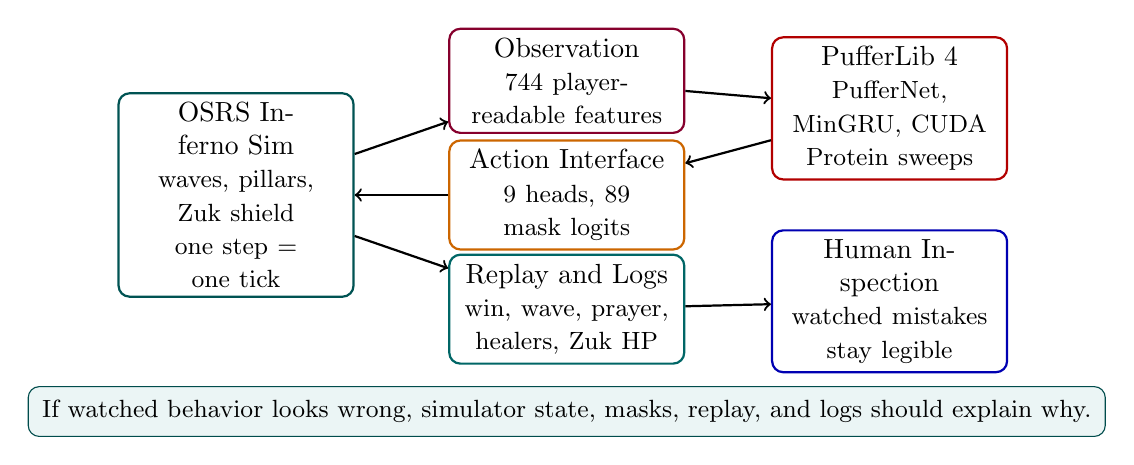
\begin{tikzpicture}[
  box/.style={draw, rounded corners, thick, align=center, text width=2.75cm, minimum height=1.0cm, fill=white},
  arrow/.style={->, thick}
]
\node[box, draw=teal!65!black, minimum height=1.45cm] (sim) at (0,0) {OSRS Inferno Sim\\{\small waves, pillars, Zuk shield}\\{\small one step = one tick}};
\node[box, draw=purple!70!black] (obs) at (4.2,1.45) {Observation\\{\small 744 player-readable features}};
\node[box, draw=orange!80!black] (act) at (4.2,0) {Action Interface\\{\small 9 heads, 89 mask logits}};
\node[box, draw=teal!80!black] (log) at (4.2,-1.45) {Replay and Logs\\{\small win, wave, prayer, healers, Zuk HP}};
\node[box, draw=red!70!black, minimum height=1.45cm] (train) at (8.3,1.1) {PufferLib 4\\{\small PufferNet, MinGRU, CUDA}\\{\small Protein sweeps}};
\node[box, draw=blue!70!black, minimum height=1.25cm] (watch) at (8.3,-1.35) {Human Inspection\\{\small watched mistakes stay legible}};
\draw[arrow] (sim) -- (obs);
\draw[arrow] (obs) -- (train);
\draw[arrow] (train) -- (act);
\draw[arrow] (act) -- (sim);
\draw[arrow] (sim) -- (log);
\draw[arrow] (log) -- (watch);
\node[align=center, fill=teal!8, draw=teal!60!black, rounded corners, inner sep=5pt] at (4.2,-2.75) {\small If watched behavior looks wrong, simulator state, masks, replay, and logs should explain why.};
\end{tikzpicture}
}
\caption{The benchmark contract. The policy trains on symbolic state and structured masks, while replay and logs expose the same facts for human inspection.}
\label{fig:contract}
\end{figure}

\section{Training and Iteration Loop}

PufferLib 4 matters here because the bottleneck is the full edit-train-watch loop. The public Puffer docs describe a native backend with CUDA C kernels, static memory, CUDA graphs, async environment workers, fused operations, action masks, PufferNet policies, and Protein sweeps \cite{puffer-docs}. Joseph Suarez's Puffer 4 engineering notes frame the same systems problem: small-model RL can spend too much time in framework overhead unless memory layout, kernel launch overhead, and fused computation are designed together \cite{puffer4-systems}.

The recurrent model is PufferNet, which combines MinGRU with highway-style output mixing. MinGRU supports parallel-scan training across sequences and cheap recurrent inference during rollouts \cite{puffernet, mingru}. That is a good fit for game tasks where the policy needs memory during rollout, but training must still use long enough sequences to learn delayed consequences.

The Inferno config uses 4096 parallel agents, two rollout buffers, 16 worker threads, a two-layer 512 hidden PufferNet, a 16 tick horizon, priority replay, and a replay ratio of 4. The horizon covers 9.6 seconds of game time. Protein sweeps search over learning rate, horizon, discounting, advantage settings, replay, vector size, model width, curriculum fractions, and reward weights. Protein models both score and wall-clock cost, which matters because a high score from a slow or unstable setting may be a poor development tool \cite{constellation}.

The hardest engineering lesson was that the simulator and learner could not be debugged separately. Training exposed missing observations, stale masks, and reward traps. Renderer checks exposed bugs in projectile anchoring, Zuk pathing, healer tags, and action timing. Human controls exposed when the action interface was not playable. The useful loop became: train, watch, find a player-readable failure, trace the simulator, add a contract test, and sweep again.

\begin{table}[t]
\centering
\small
\begin{tabular}{lll}
\toprule
Observed failure & Visible signal & Contract added \\
\midrule
Wrong prayer timing & Prayer correctness and death context & Pending-hit observations \\
Stale target options & Zero-valid-head counters & Strict target masks \\
Missed Zuk healers & Healer tag and kill logs & Healer phase diagnostics \\
Broken Zuk movement & Replay and human click pathing & Shield-path checks \\
Wrong projectile source & Rendered flight path & Anchored projectile endpoints \\
\bottomrule
\end{tabular}
\caption{Examples where policy watching, metrics, and simulator contracts found different classes of defect.}
\label{tab:failures}
\end{table}

\section{Checkpoint Evidence}

The current checkpoint result is a compact recurrent policy trained in the active development branch. It uses the compact Redemption overhead mapping, state curriculum, priority replay, 4096 parallel agents, a two-layer 512 hidden PufferNet, and 171.7M environment steps. The stored run summary reports the development telemetry in Table \ref{tab:result}. The summary marks the final metrics as normal-start evaluation, but this artifact is downsampled, so we avoid treating its \texttt{env/n} field as a precise evaluation denominator here.

\begin{table}[t]
\centering
\small
\begin{tabular}{lr}
\toprule
Metric & Value \\
\midrule
Environment steps & 171.7M \\
Logged win rate & 0.489635 \\
Internal progress score & 0.736389 \\
Average final wave & 66.720871 \\
Average minimum Zuk HP on failed runs & 240.535599 \\
Prayer correctness & 0.853395 \\
Fraction reaching Zuk healers & 0.847019 \\
Fraction killing all Zuk healers & 0.718624 \\
Final logged throughput & about 256k steps/s \\
\bottomrule
\end{tabular}
\caption{Stored development telemetry for the compact recurrent Inferno checkpoint.}
\label{tab:result}
\end{table}

These numbers should be read with care. The environment, action surface, and visual contract were still changing during development. The result shows that the current benchmark version can train a policy that clears the full encounter and reaches late-Zuk states often. It does not prove that the task is solved, that the checkpoint is robust across future environment versions, or that the policy has no simulator-specific habits.

This distinction is central to the benchmark. In an inspectable game task, success cannot be only a scalar. A policy that clears while wasting supplies, mistiming healers, or leaning on a simulator bug has not solved the benchmark in the player-facing sense. The benchmark should keep these failures visible.

A stricter public benchmark release should do more than run more episodes. It should freeze the observation and action schema, pin the checkpoint metadata, run normal-start no-render evaluation with an explicit episode count, replay sampled wins and losses, and report behavioral counters alongside score. A policy should be judged on full clears, late-phase progress, and whether watched failures remain explainable from logged state.

\section{Lessons and Limitations}

First, game benchmarks need a player-facing contract. If policy behavior looks wrong in replay, the logs and simulator should explain why. This is not a cosmetic requirement. In the Inferno, rendering and replay caught bugs that scalar training curves would have hidden.

Second, strict action masks are part of the task definition. OSRS has many impossible actions: attacking missing targets, drinking empty potions, casting unavailable spells, switching to already equipped gear, or stepping into blocked tiles. Masking these actions does not make the game easy. It removes interface noise so the model can spend capacity on game decisions.

Third, reward is not score. Reward is an engineering tool for credit assignment. Score is the stable development yardstick. Keeping them separate made the project less brittle while reward weights and curricula changed.

Fourth, higher throughput made the development loop more empirical. PufferLib 4's static memory, fused kernels, CUDA graphs, MinGRU, and sweep tooling were not aesthetic choices. They made it cheap enough to find out whether a simulator fix or observation change actually helped \cite{puffer4-systems, puffernet, constellation}.

The main limitation is fidelity. This is not a full OSRS client. It is a simulator for the encounter mechanics that matter for training, plus cache-derived assets for visual inspection. Expert knowledge makes failures interpretable, but it can also hide assumptions in the simulator. The safest path is to keep tests, render checks, replay checks, and human play close to the training surface.

The OSRS Inferno environment suggests a benchmark pattern for long-horizon game RL: player-readable state, structured actions, strict masks, replayable failures, and high-throughput recurrent training. A benchmark should report whether an agent wins and make the agent's mistakes legible.

\small
\begin{thebibliography}{9}
\bibitem{osrs-inferno} OSRS Wiki. Inferno. \url{https://oldschool.runescape.wiki/w/Inferno}
\bibitem{puffer-docs} PufferAI. PufferLib docs. \url{https://puffer.ai/docs.html}
\bibitem{puffer4-systems} Joseph Suarez. The Engineering behind PufferLib 4.0's 20,000,000 step/second RL Training. \url{https://x.com/jsuarez/article/2041501879222284776}
\bibitem{puffernet} Joseph Suarez. A High Throughput Recurrent Network for PufferLib 4.0. \url{https://x.com/jsuarez/article/2042273938592407674}
\bibitem{mingru} Feng et al. Were RNNs All We Needed? arXiv:2410.01201. \url{https://arxiv.org/abs/2410.01201}
\bibitem{constellation} Joseph Suarez. Visualizing 20k RL Experiments with Constellation. \url{https://x.com/jsuarez/article/2041896392587722885}
\bibitem{pufferlib-paper} Suarez. PufferLib: Making Reinforcement Learning Libraries and Environments Play Nice. arXiv:2406.12905. \url{https://arxiv.org/abs/2406.12905}
\end{thebibliography}

\end{document}
